\subsubsection{Plux.NET}

{\it Plux.NET} --- платформа для работы с плагинами для {\tt .NET}, позволяющая создавать расширяемые приложения, состоящие из <<ядра>>, содержащего минимальный набор функций и возможностей, и набора расширений. В терминологии {\it Plux.NET} ядро --- это основное приложение (host). В ядре содержится набор слотов. Слот определяется как некий контракт между хост-приложением и расширениями, которые могут <<вставляться>> в слот. Загрузка расширений происходит во время выполнения программы. 

В простейшем случае, слот определяет интерфейс, а также набор параметров с типами. Расширение предоставляет реализацию этого интерфейса вместе со списком значений требуемых параметров. Хост-приложение  будет использовать эти параметры для загрузки и интеграции расширения. Слоты и расширения описываются в виде атрибутов {\tt .NET}.

Для примера описанной концепции рассмотрим абстрактное приложение с графическим пользовательским интерфейсом, которое позволяет в зависимости от установленных расширений добавлять новые команды в меню. Основное приложение <<открывает>> слот, описывая интерфейс {\tt IMenuItem} и два параметра: {\tt Text} (название элемента меню) и {\tt Icon} (пиктограмма пункта меню). Расширение --- это класс, реализующий интерфейс {\tt IMenuItem}, а также значения параметров (к примеру, <<Print>> в качестве названия элемента меню и графический файл <<Print.jpg>> в качестве пиктограммы). На рисунке \ref{plux-scheme} показана схема взаимодействия основного приложения с открытым слотом и расширения:

\begin{figure}[!h]
    \centering
    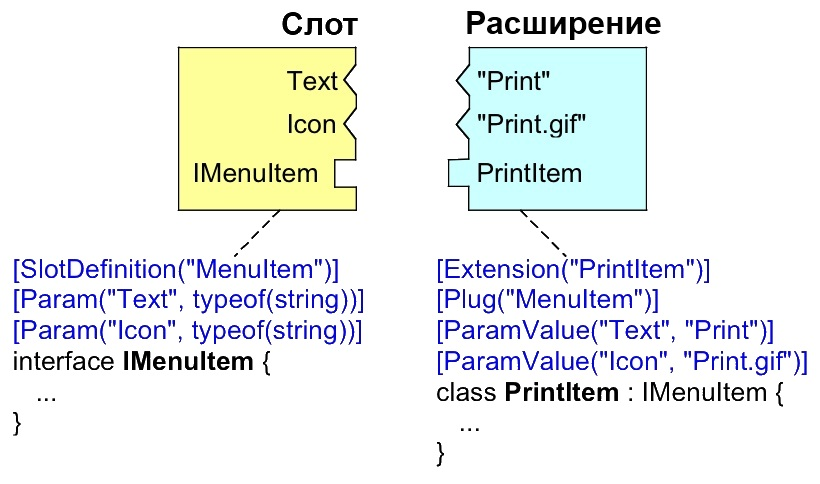
\includegraphics[width=12cm]{plux1.jpg}
    \caption{Подключение расширения к слоту в платформе Plux.NET}
    \label{plux-scheme}
\end{figure}


Для каждого открытого слота платформа {\it Plux.NET} определяет доступные подходящие расширения, загружает их, присваивает значения параметрам и уведомляет хост-приложение о подключении расширения к слоту. После этого хост-приложение предпринимает действия по интеграции расширения (в примере с приложением с графическим пользовательским интерфейсом, добавляя пункты в меню и устанавливая обработчики событий).